\documentclass[]{article}

\usepackage[italian]{babel}
\usepackage[margin=20mm, footskip = 20pt]{geometry}
\usepackage{array}
\usepackage{tabularx}
\usepackage{graphicx}
\usepackage{subfiles}
\usepackage{hyperref}
\usepackage{nameref}
\usepackage{titlesec}
\usepackage{longtable}
\usepackage[table]{xcolor}
\usepackage{titling}
\usepackage{lastpage}
\usepackage{ifthen}
\usepackage{calc}
\usepackage{soulutf8}
\usepackage{contour}
\usepackage{float}
\usepackage{fancyhdr}
\usepackage{multirow}
\usepackage{pgfgantt}
\usepackage{lscape}

\newcommand{\hr}{\par\vspace{-.1\ht\strutbox}\noindent\hrulefill\par}

\graphicspath{ {./}
	{./commons/res}
}

%--------------------------------------------------
% Comandi per inserire contenuto del documento
%--------------------------------------------------
\makeatletter

\newcommand\appendToGraphicsPath[1]{%
	\g@addto@macro\Ginput@path{{#1}}%
}

\newcommand{\setTitle}[1]{%
	\newcommand{\@phTitle}{#1}%
}
\newcommand{\phTitle}{\@phTitle}

\newcommand{\setDate}[1]{%
	\newcommand{\@phDate}{#1}%
}
\newcommand{\phDate}{\@phDate}

\newcommand{\setUso}[1]{%
	\newcommand{\@uso}{#1}%
}
\newcommand{\uso}{\@uso}

\newcommand{\setVersione}[1]{%
	\newcommand{\@versione}{#1}%
}
\newcommand{\versione}{\@versione}

\newcommand{\disabilitaVersione}{%
	\renewcommand{\setVersione}[1]{}%
	\renewcommand{\versione}{DISABILITATA}
}

\newcommand{\setResponsabile}[1]{%
	\newcommand{\@responsabile}{#1}%
}
\newcommand{\responsabile}{\@responsabile}

\newcommand{\setRedattori}[1]{%
	\newcommand{\@redattori}{#1}%
}
\newcommand{\redattori}{\@redattori}

\newcommand{\setVerificatori}[1]{%
	\newcommand{\@verificatori}{#1}%
}
\newcommand{\verificatori}{\@verificatori}

\newcommand{\setModifiche}[1]{%
	\newcommand{\@modifiche}{#1}%
}
\newcommand{\modifiche}{\@modifiche}

\makeatother 

%--------------------------------------------------
% Comandi per i documenti esterni e il glossario
%--------------------------------------------------

\newcommand{\dext}[1]{\textsc{#1\textsubscript{\textit{D}}}}

\newcommand{\glock}[1]{\textsc{#1\textsubscript{\textit{G}}}}

%--------------------------------------------------
% Comandi per impostare sottotitoli di quarto e quinto livello
%--------------------------------------------------

\setcounter{secnumdepth}{4}
\setcounter{tocdepth}{4}

\titleformat{\paragraph}
{\normalfont\normalsize\bfseries}{\theparagraph}{1em}{}
\titlespacing*{\paragraph}{0pt}{2.25ex plus 1ex minus .2ex}{1.5ex plus .2ex}

\titleformat{\subparagraph}
{\normalfont\normalsize\bfseries}{\thesubparagraph}{1em}{}
\titlespacing*{\subparagraph}{0pt}{1.75ex plus 1ex minus .2ex}{.75ex plus .1ex}

\appendToGraphicsPath{../../../commons/res/}

%------------------------------
%
% COMANDI DI CONFIGURAZIONE
%
%------------------------------

\setTitle{Verbale esterno \#7}

\setVersione{0.1.0}

\setDate{13-04-2021}

\setResponsabile{Alessandro Chimetto}

\setRedattori{Matteo Alba}

\setVerificatori{Alessandro Dindinelli}

\setUso{Esterno}

\setModifiche{
	0.1.0 & Alessandro Dindinelli & Verificatore & 20-05-2021 & Verifica documento \\
	0.0.0 & Matteo Alba & Amministratore & 13-04-2021 & Stesura iniziale}

\begin{document}

	% Direttive per la creazione del titolo tramite comando maketitle
\title{\huge \textsc{\phTitle{}} \\
	\vspace{11pt} \large \textsc{\phDate{}}}

\author{} % Non toccare
\date{} % Non toccare

%--------------------
% Frontespizio
%--------------------

% Logo del gruppo
\begin{figure}[t!]
	\centering
	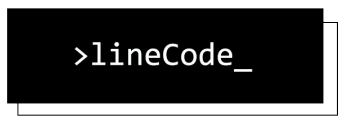
\includegraphics[width=20em]{lclong}
\end{figure}

% Titolo / Nome
\maketitle
\thispagestyle{empty}

% Dati specifici sul doc in forma tabulare
\begin{table}[ht]
	\begin{center}
		\label{tab:Dati sul documento}
		\begin{tabular}{r|l}
			\multicolumn{2}{c}{ \textsc{Dati sul documento} } \\
			\hline
			\textbf{Versione} & \versione{} \\
			\textbf{Uso} & \uso{}  \\
			\textbf{Redattori} & \redattori{} \\
			\textbf{Verificatori} & \verificatori{} \\
			\textbf{Responsabile} & \responsabile{} \\
			\textbf{Destinatari} & lineCode \\
								& prof.\ Vardanega Tullio \\		
								& prof.\ Cardin Riccardo \\
			\ifthenelse{\equal{\uso}{Esterno}}{
								& Sanmarco Informatica
			}{} \\
		\end{tabular}
	\end{center}
\end{table}

\newpage

\renewcommand{\arraystretch}{2} % allarga le righe con dello spazio sotto e sopra
\begin{longtable}[H]{>{\centering\bfseries}m{2cm} >{\centering}m{3.5cm} >{\centering}m{2.5cm} >{\centering}m{3cm} >{\centering\arraybackslash}m{5cm}}
	\rowcolor{lightgray}
	{\textbf{Versione}} & {\textbf{Nominativo}} & {\textbf{Ruolo}} & {\textbf{Data}} & {\textbf{Descrizione}}  \\
	\endfirsthead%
	\rowcolor{lightgray}
	{\textbf{Versione}} & {\textbf{Nominativo}}  & {\textbf{Ruolo}} & {\textbf{Data}} & {\textbf{Descrizione}}  \\
	\endhead%
	\modifiche{}%
\end{longtable}

	\newpage

	%--------------------------------
	%
	% IL CONTENUTO INIZIA DA QUI
	%
	%--------------------------------

	\section{Introduzione}
	\subsection{Luogo e data dell'incontro}
	\begin{itemize}
		\item \textbf{Modalità}: Telematica;
		\item \textbf{Software utilizzato}: Google Meet;
		\item \textbf{Data}: 12 Aprile 2021;
		\item \textbf{Ora di inizio}: 15:00;
		\item \textbf{Ora di fine}: 16:00.
	\end{itemize}

	\subsection{Presenze}
	\begin{itemize}
		\item \textbf{Presenti}:
		\begin{itemize}
			\item Matteo Alba			
			\item Alessandro Chimetto
			\item Alessandro Dindinelli
			\item Paolo Scanferlato

		\end{itemize}
		\item \textbf{Assenti}:
		\begin{itemize}
			\item Valton Tahiraj
			\item Lucia Fenu
			\item Giacomo Bulbarelli

		\end{itemize}
		\item \textbf{Partecipanti esterni}:
		\begin{itemize}
			\item Alex Beggiato (referente, Sanmarco Informatica)
		\end{itemize}
	\end{itemize}

	\subsection{Ordine del giorno}
	\begin{enumerate}
		\item Discussione degli ultimi dubbi prima della revisione.
	\end{enumerate}
	\newpage
	\section{Svolgimento}


	\subsection{Discussione degli ultimi dubbi prima della revisione}
	Durante l'incontro si è parlato brevemente della UI ma ci si è maggiormente dedicati alla parte relativa all'architettura del server. 
	In particolare il punto focale della discussione è stata la suddivisione dei layer ed il passaggio dei dati da uno all'altro, affrontando il problema della legge di Demetra.
	Il consiglio del relatore è stato quello di incapsulare la parte di anagrafica in modo tale che il passaggio dei dati risulti minimale.
	L'ultima parte dell'incontro è stata relativa alla configurazione del Business Layer, ed è stato deciso dal gruppo che era fondamentale utilizzare un singleton che contiene un riferimento ai servizi evitando strutture dati statiche ed avere un'istanza singola per ogni servizio.
	Ci è stato poi suggerito di richiamare il singleton all'interno delle classi con l'enumeration ma dopo averne discusso con il gruppo abbiamo deciso di non utilizzarlo e di proseguire come stavamo già facendo perchè ci sembrava più adatto al nostro scopo.
	In generale la realizzazione dell'architettura è stata apprezzata.

	\newpage

	\section{Tabella delle decisioni}

	\begin{table} [h!]
		\rowcolors{2}{gray!25}{gray!6}
		\begin{center}
			\begin{tabular} { m{2cm} m{14cm} }
				\rowcolor{lightgray}
				\textbf{ID} & \textbf{Decisione}\\
				VE_2021-04-12_7.1 & Si è deciso di utilizzare un singleton per evitare la dipendenza circolare nell'architettura del server.
			\end{tabular}
		\end{center}
	\end{table}
\end{document}

